\section{Atrito}
    A força de atrito deve-se à existência de rugosidades na 
superfície de contato do objeto com o solo. Essas rugosidades não são observadas 
macroscopicamente, mas são elas que dificultam o movimento\cite{da2019estudo}.


\begin{figure}[ht]
    \centering
    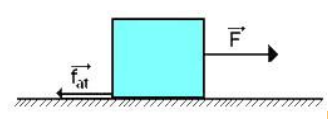
\includegraphics{JoseGeraldo-lista1/fig/fig1.png}
    \caption{bloco com atrito}
    
    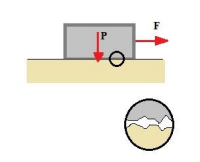
\includegraphics{JoseGeraldo-lista1/fig/fig2.png}
    \caption{Rugosidades}
\end{figure}


\textbf{Atrito Estático:} é aquele que atua quando não há deslizamento dos corpos. 
A força de atrito estático máxima é igual à força mínima necessária para iniciar o 
movimento de um corpo. Quando um corpo não está em movimento à força de atrito 
deve ser maior que a força aplicada, neste caso, é usado no cálculo um coeficiente 
de atrito estático. A força de atrito estático é descrita pela seguinte equação\cite{da2019estudo}.
\begin{equation}
            F_{a_t} = µ_e \times N
            \label{equ:Atrito estatico}
\end{equation}

\textbf{Atrito Dinâmico:} é aquele que tem deslizamento dos corpos. Quando a força 
de atrito estático for ultrapassada pela força aplicada ao corpo, este entrará em 
movimento, e passaremos a considerar sua força de atrito dinâmico. A força de atrito 
dinâmico é sempre menor que a força aplicada, no seu cálculo é utilizado o 
coeficiente de atrito cinético. A equação a seguir descreve a F de atrito dinâmico\cite{da2019estudo}.
\begin{equation}
            F_{a_t} = µ_d \times N
            \label{equ:Atrito dinamico}
\end{equation}

\section{Polias e Roldanas}
Polias ou roldanas são dispositivos mecânicos usados para tornar mais cômodo ou reduzir a força necessária para deslocar objetos com um grande peso.

Esse tipo de máquina simples é composta por uma ou mais rodas, que giram em torno de um eixo central e possui um sulco por onde passa uma corda ou fio flexível\cite{site1}.

\textbf{Roldanas Fixas:} A roldana fixa tem o seu eixo preso em algum ponto apoio, portanto, apresenta apenas movimento de rotação, não sendo possível o movimento de translação.
Elas modificam apenas o sentido e a direção da força motora que equilibra o peso. Desta forma, são utilizadas para tornar mais cômodo o trabalho de puxar um objeto.
Nas roldanas fixas não verificamos uma redução no esforço necessário para movimentar um objeto. Portanto, o módulo da força motora será igual ao módulo da força resistente (peso da carga a ser transportada)\cite{site1}.

\begin{figure}[ht]
    \centering
    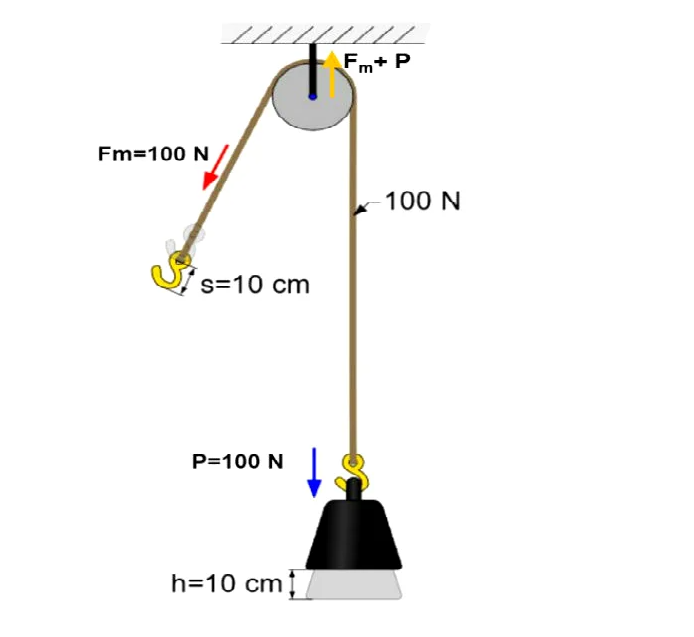
\includegraphics[scale=0.5]{JoseGeraldo-lista1/fig/fig4.png}
    \caption{Exemplo de forças que atuam no movimento de uma roldana fixa}
\end{figure}


\textbf{Roldanas Moveis:} Diferente das roldanas fixas, as móveis possuem o eixo livre, desta maneira, possuem movimento de rotação e também de translação.
A força resistente que deve ser equilibrada encontra-se no eixo da roldana, enquanto a força motora é aplicada no extremo livre da corda.
A grande vantagem do uso das roldanas móveis é que reduz o valor da força motora necessária para movimentar um determinado corpo, entretanto, um comprimento maior de corda deverá ser puxado\cite{site1}.
\begin{figure}[ht]
    \centering
    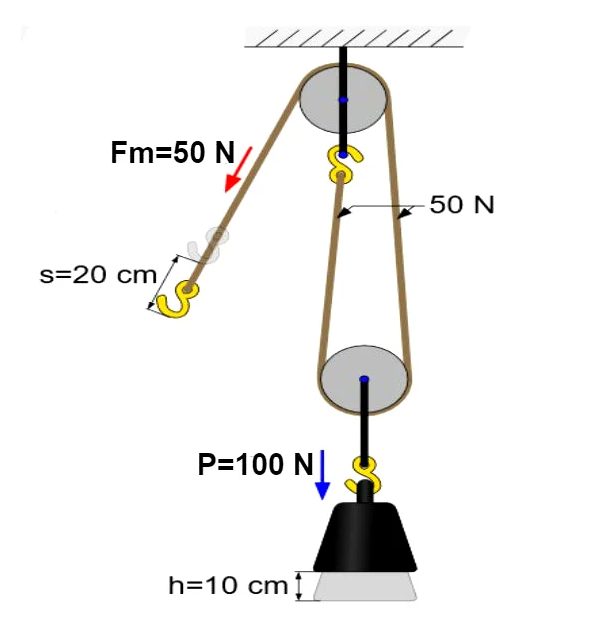
\includegraphics[scale=0.7]{JoseGeraldo-lista1/fig/fig5.png}
    \caption{Exemplo de forças que atuam no movimento de uma roldana móvel}
\end{figure}